% Created 2014-12-13 Sat 15:20
\documentclass{article}
\usepackage[top=1in, bottom=1.in, left=1in, right=1in]{geometry}
  

\usepackage[utf8]{inputenc}
\usepackage{lmodern}
\usepackage[T1]{fontenc}
\usepackage{fixltx2e}
\usepackage{graphicx}
\usepackage{longtable}
\usepackage{float}
\usepackage{wrapfig}
\usepackage{rotating}
\usepackage[normalem]{ulem}
\usepackage{amsmath}
\usepackage{textcomp}
\usepackage{marvosym}
\usepackage{wasysym}
\usepackage{amssymb}
\usepackage{amsmath}
\usepackage[version=3]{mhchem}
\usepackage[numbers,super,sort&compress]{natbib}
\usepackage{natmove}
\usepackage{url}
\usepackage{minted}
\usepackage{underscore}
\usepackage[linktocpage,pdfstartview=FitH,colorlinks,
linkcolor=blue,anchorcolor=blue,
citecolor=blue,filecolor=blue,menucolor=blue,urlcolor=blue]{hyperref}
\usepackage{attachfile}
\author{Prateek Mehta and Hui Li}
\date{\today}
\title{Monte-Carlo Simulations of the 2-D Ising Model}
\begin{document}

\maketitle
\tableofcontents

\section{A brief note about this document}
\label{sec-1}

This document was prepared with Emacs \href{http://orgmode.org}{orgmode}. All the code was written and executed within the org-document and the results were captured in place. It has been exported into a latex \href{./ising-monte-carlo.pdf}{pdf} You can get the original org-file and all the other relevant files at this git repo: \url{https://github.com/prtkm/ising-monte-carlo}. If you are reading the pdf you can view the source by clicking here: \attachfile{ising-monte-carlo.org} (Mac Preview does not read this attachment).


\section{A reliable random number generator}
\label{sec-2}

For reliable Monte-Carlo simulations, we need a good random number generator. We shall use  Python's \texttt{numpy.random}. It uses the \emph{Mersenne twister} pseudo-random number generator, so we should expect to get a uniform random distribution. We test this here. Let us generate a 10000 random numbers and plot them.

\begin{minted}[frame=lines,fontsize=\scriptsize,linenos]{python}
import numpy as np
import matplotlib.pyplot as plt

plt.plot(range(10000), np.random.random(10000), '.')
plt.savefig('images/numpy-random.png')
plt.show()
\end{minted}

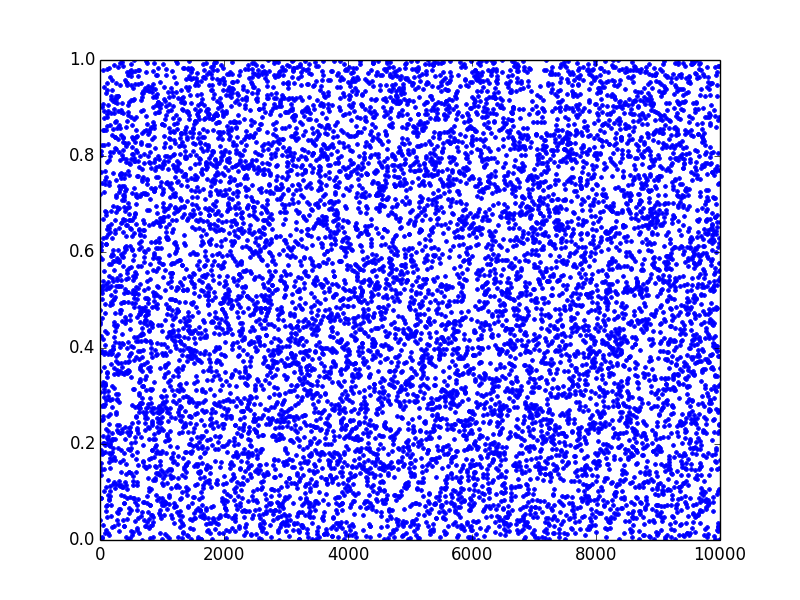
\includegraphics[width=.9\linewidth]{./images/numpy-random.png}

That looks pretty uniform!



\section{2-D Ising Model Simulator}
\label{sec-3}

The main ideas to simulate the 2-D Ising Model using Metropolis Monte Carlo are as follows:

\begin{itemize}
\item We create a n \texttimes{} n lattice with a random spin configuration

\item For the purposes of our Monte Carlo simulation we start off by randomly flipping a spin and calculate the change in energy, $\Delta$ E

\item If $\Delta$ E is negative, we accept the new configuration and move to the next step

\item If $\Delta$ E is positive, we select a random number between 0 and 1, and accept the configuration only if the number is less than \(e^{-\Delta E / k_{B}T}\). This is the Metropolis techinque. This saves computation time by selecting the more probable configurations.

\item We use periodic boundary conditions. This effectively reduces the geometry of the problem to a torus.

\item To simulate over a range of temperatures, we will submit jobs to the queue system for every temperature.  This is useful, especially for large lattice sizes where a lot of simulations are required to reach convergence. We have found that at large lattices flipping one spin per step is pretty inefficient (for a 1000 \texttimes{} 1000 lattice, we are practically flipping one spin in a million!). A better approach than ours is probably needed in such cases, maybe flipping multiple spins at the same time.
\end{itemize}

Here is our main script that does all the work. We write this out to our system for use later.
\begin{minted}[frame=lines,fontsize=\scriptsize,linenos]{python}
from __future__ import division
import numpy as np

def init_lattice(n):

    '''Create a nxn lattice with random spin configuration'''
    
    lattice = np.random.choice([1, -1], size=(n, n))
    return lattice


def deltaE(S0, Sn, J, H):

    '''Energy difference for a spin flip'''
    
    return 2 * S0 * (H + J * Sn)


def ising(n=200, 
          nsteps=500000,
          H=0,
          J=1,
          T=1,
          count_spins = False,
          countij = [1,1],
          correlation=False,
          corr_ij=[0,0],
          corr_r=1):

    '''Ising Model Simulator. If count_spins = True, only flipping behavior of 1 site is studied.'''
    
    lattice = init_lattice(n)
    energy = 0
    energies = []
    spins = []
    spin = np.sum(lattice)
    icount, jcount = countij
    counted_spins = [lattice[icount, jcount]]
    counted_intervals = []
    icorr, jcorr = corr_ij
    Sis = []
    SiSjs = []
    
    for step in xrange(nsteps):

        i = np.random.randint(n)
        j = np.random.randint(n)

        # Periodic Boundary Condition
        Sn = lattice[(i - 1) % n, j] + lattice[(i + 1) % n, j] + \
             lattice[i, (j - 1) % n] + lattice[i, (j + 1) % n]

        dE = deltaE(lattice[i, j], Sn, J, H)

        if dE < 0 or np.random.random() < np.exp(-dE/T):
            lattice[i, j] = -lattice[i, j]
            energy += dE
            energies.append(energy)
         # Note that the spin is collected at every step
            spin += 2*lattice[i, j]
        
        if count_spins:
            ispin = lattice[icount, jcount]
            if ispin != counted_spins[-1]:
                counted_spins.append(ispin)
                counted_interval = step - sum(counted_intervals)

                counted_intervals.append(counted_interval)
        if correlation:
            Sn_corr = lattice[(icorr - corr_r) % n, jcorr] + lattice[(icorr + corr_r) % n, jcorr] + \
                      lattice[icorr, (jcorr - corr_r) % n] + lattice[icorr, (jcorr + corr_r) % n]
            Si = lattice[icorr, jcorr]
            SiSj = Si * Sn_corr / 4.0
            Sis.append(Si)
            SiSjs.append(SiSj)
            
        spins.append(spin)


    if correlation:
        return Sis, SiSjs
    
    if count_spins:
        return counted_spins, counted_intervals
        
    return lattice, energies, spins
    

def ising1000(n=1000, nsteps=10000000000, H=0, J=1, T=1):

    '''Ising Model Simulator. Special case for very large lattices.
    To reduce some memory usage:
    spin is added to the array every 1000 steps.
    Energies are not returned.
    Still pretty inefficient!
    '''
    
    lattice = init_lattice(n)
    energy = 0

    spins = []
    spin = np.sum(lattice)
    for istep, step in enumerate(xrange(nsteps)):

        i = np.random.randint(n)
        j = np.random.randint(n)

        # Periodic Boundary Condition
        Sn = lattice[(i - 1) % n, j] + lattice[(i + 1) % n, j] + \
             lattice[i, (j - 1) % n] + lattice[i, (j + 1) % n]

        dE = deltaE(lattice[i, j], Sn, J, H)

        if dE < 0 or np.random.random() < np.exp(-dE/T):
            lattice[i, j] = -lattice[i, j]
            energy += dE
            spin += 2*lattice[i, j]
        if istep % 1000 == 0:
            spins.append(spin)
    return lattice, spins


def write_job_script(wd='./', n=10, s=1000, i=1, T=1., nprocs=1, pe='smp', name = 'batch', q = 'long'):
    '''
    This is a function that writes a script to submit MC jobs
    '''
    py_file = '/afs/crc.nd.edu/user/p/pmehta1/ising-monte-carlo/spins.py'
    script='''#!/bin/bash
#$ -N {0}
#$ -pe {1} {2}
#$ -q {3}
#$ -cwd
'''.format(name, pe, nprocs, q)
       
    if nprocs > 1:
        cmd = 'mpirun -np $NSLOTS python'
        script+='{6} {5} -n {0} -s {1} -i {2} -t {3} -w {4}'.format(n, s, i, T, wd, py_file, cmd)

    else:
        script+='python {5} -n {0} -s {1} -i {2} -t {3} -w {4}'.format(n, s, i, T, wd, py_file)

    with open('{0}/qscript'.format(wd), 'w') as f:
        f.write(script)

def run_job(wd):
    '''
    Submit job to the queue
    '''
    import os
    from subprocess import Popen, PIPE
    cwd = os.getcwd()
    os.chdir(wd)
    p = Popen(['qsub', 'qscript'], stdout=PIPE, stderr=PIPE)
    out, err = p.communicate()
    
    if out == '' or err !='':
        raise Exception('something went wrong in qsub:\n\n{0}'.format(err))
    jobid = out.split()[2]
    f = open('jobid', 'w')
  
    f.write(jobid)
    f.close()
    os.chdir(cwd)
    return out.strip()
\end{minted}


\section{Average Spin Trajectories}
\label{sec-4}

Now we plot the average spin trajectories at three different temperatures. The spin is collected at every step of the Monte Carlo simulation, regardless of whether we accepted the flip or not.

\begin{minted}[frame=lines,fontsize=\scriptsize,linenos]{python}
import matplotlib.pyplot as plt
from ising import *

temperatures = [0.5, 2.27, 5.0]

for T in temperatures:

    lattice, energies, spins = ising(n=20, nsteps = 500000, T=T)
    spins = np.array(spins) / 20. ** 2
    plt.plot(range(len(spins)), spins, label = 'T = {0}'.format(T))
plt.legend(loc = 'best')
plt.xlabel('nSteps')
plt.ylabel('Average Spin')
plt.ylim(-1.2, 1.2)
plt.savefig('images/average-spin.png')
plt.show()
\end{minted}

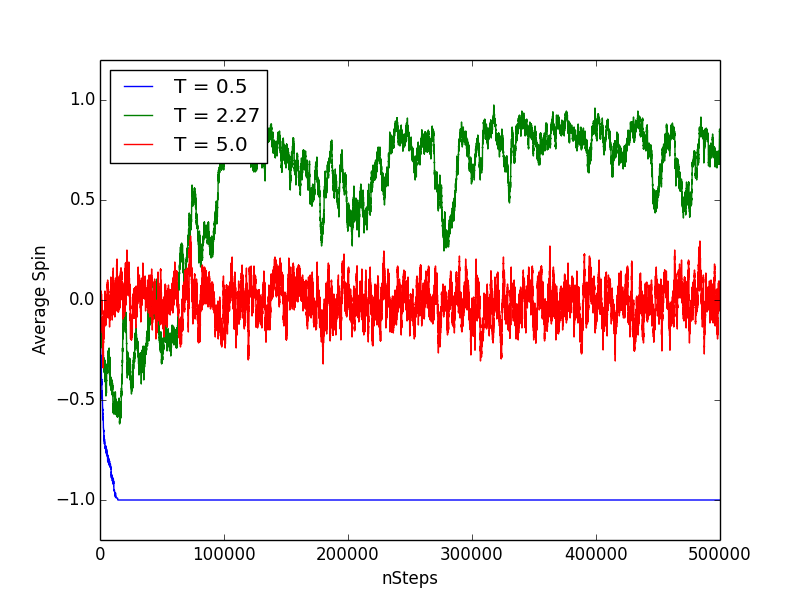
\includegraphics[width=.9\linewidth]{./images/average-spin.png}

This looks pretty much like what one would expect. At a low temperature the average spin per site is 1, meaning that all the points in the lattice have the same spin. At a temperature close to Onsager's T$_{\text{c}}$, the system has an intermediate spin, and at a high temperature, the system has no net spin. 



\section{Magnetization and Susceptibility}
\label{sec-5}
In this section, we calculate the magnetization and susceptibility at different lattice sizes and temperatures. 

\subsection{Submission to the queue}
\label{sec-5-1}

To simulate things for multiple temperatures and lattice sizes, we submited jobs to the queueing system. This is the python script that we will execute in the queue.

\begin{minted}[frame=lines,fontsize=\scriptsize,linenos]{python}
#!/usr/bin/env python
import os
from ising import ising, ising1000
import sys,getopt
opts,args = getopt.getopt(sys.argv[1:],'n:s:i:t:w')

for key, val in opts:

    if key == '-n': n = int(val)
    elif key == '-s': nsteps = int(val)
    elif key == '-t': T = float(val)
    elif key == '-i': index = int(val)
    elif key == '-w': wd = str(val)

if n < 500:
    lattice, energies, spins = ising(n=n, nsteps=nsteps, T=T)
else:
    lattice, spins = ising1000(n=n, nsteps=nsteps, T=T)
    
with open(os.path.join(wd,'temp-{1}.out'.format(wd, index)), 'w') as f:
    for i, spin in enumerate(spins):
        if i % 1000 == 0:
            f.write("{0}\t{1}\n".format(i, spin))
\end{minted}

We submit jobs here for multiple lattice sizes and temperatures.

\begin{minted}[frame=lines,fontsize=\scriptsize,linenos]{python}
from ising import *
import os

Ns = [10, 20, 50, 100, 1000]  # System Size
T_Tcs = np.linspace(0.5, 1.7, 30)  # T/Tc
Tc = 2.268  # Onsager's Tc

for n in Ns:
    for i, T_Tc in enumerate(T_Tcs):
        T = T_Tc*Tc
        wd = 'magnetization/size-{0}/temp-{1}'.format(n, i)
        if not os.path.exists(wd): 
            os.makedirs(wd)
        if n !=1000:
            write_job_script(wd=wd, n=n, s= n * 1000000, T=T, i=i)
        else:
            write_job_script(wd=wd, n=n, s= n * 1000000, T=T, i=i, nprocs = 1, q ='long')
        run_job(wd)
\end{minted}

\subsection{Magnetization}
\label{sec-5-2}
Here we plot the magnetization. We see that for larger lattice sizes, the system has not reached equilibirum and the data is very noisy. Otherwise the plot matches what is known, i.e, full magnetization at low temperatures, disorder at higher temperatures, with a transition at the critical temperature. The transition is sharper at larger lattice sizes. 

\begin{minted}[frame=lines,fontsize=\scriptsize,linenos]{python}
from __future__ import division
import matplotlib.pyplot as plt
from ising import *
import os

Ns = [10, 20, 50, 100, 1000]  # System Size
T_Tcs = np.linspace(0.5, 1.7, 30)  # T/Tc
Tc = 2.268  # Onsager's Tc

for n in Ns:
    avgspins = []
    for i, T_Tc in enumerate(T_Tcs):
        T = T_Tc*Tc
        indices, spins = np.loadtxt('magnetization/size-{0}/temp-{1}/temp-{1}.out'.format(n,i), unpack =True)
        spins = spins[int(len(spins)/2):]
        avgspin = np.sum(np.abs(spins)) / n ** 2 / len(spins)
        avgspins.append(avgspin)
    plt.plot(T_Tcs, avgspins, 'o-', label = 'L = {0}'.format(n))

plt.xlabel('T/T$_{c}$', fontsize = 16)
plt.ylabel('<M$_{L}$>', fontsize = 16)
plt.legend()
plt.savefig('images/magnetization.png')
plt.show()
\end{minted}

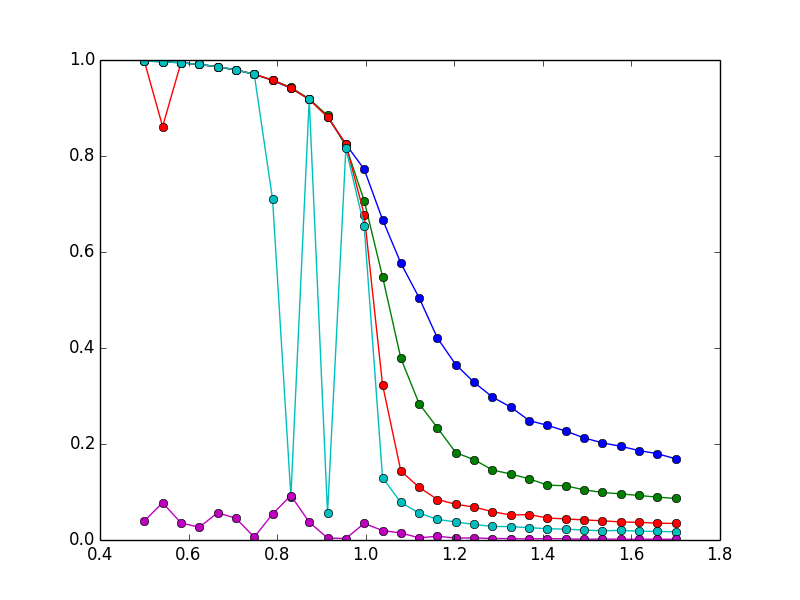
\includegraphics[width=.9\linewidth]{./images/magnetization.png}

\subsection{Susceptibility}
\label{sec-5-3}

Susceptibility is the second derivative of the energy and measures the extent to which the lattice will be magnitized. It is discontinuous at the critical temperature. We see that the peak gets sharper, and T/T$_{\text{c}}$ gets closer to unity with increasing lattice size. This means that larger lattices give better approximations of Onsager's T$_{\text{c}}$, and an inifite lattice would have exact resemblance. The data looks very noisy at high temperatures!

\begin{minted}[frame=lines,fontsize=\scriptsize,linenos]{python}
from __future__ import division
import matplotlib.pyplot as plt
from ising import *
import os

Ns = [10, 20, 50, 100, 1000]  # System Size
T_Tcs = np.linspace(0.5, 1.7, 30)  # T/Tc
Tc = 2.268  # Onsager's Tc

for n in Ns:
    avgspins = []
    Xs = []
    for i, T_Tc in enumerate(T_Tcs):
        T = T_Tc*Tc
        indices, spins = np.loadtxt('magnetization/size-{0}/temp-{1}/temp-{1}.out'.format(n,i), unpack =True)
        spins = spins[int(len(spins)/2):]
        avgspin = np.sum(np.abs(spins)) / n ** 2 / len(spins)
        X =  np.abs(np.sum(((np.abs(spins) / n ** 2) ** 2)) \
                    / len(spins) - avgspin) / T
        avgspins.append(avgspin)
        Xs.append(X)
    plt.plot(T_Tcs, Xs, 'o-', label = 'L = {0}'.format(n))
plt.xlabel('T/T$_{c}$', fontsize = 16)
plt.ylabel('$\chi$', fontsize = 16)
plt.legend()
plt.savefig('images/susseptibility.png')
plt.show()
\end{minted}

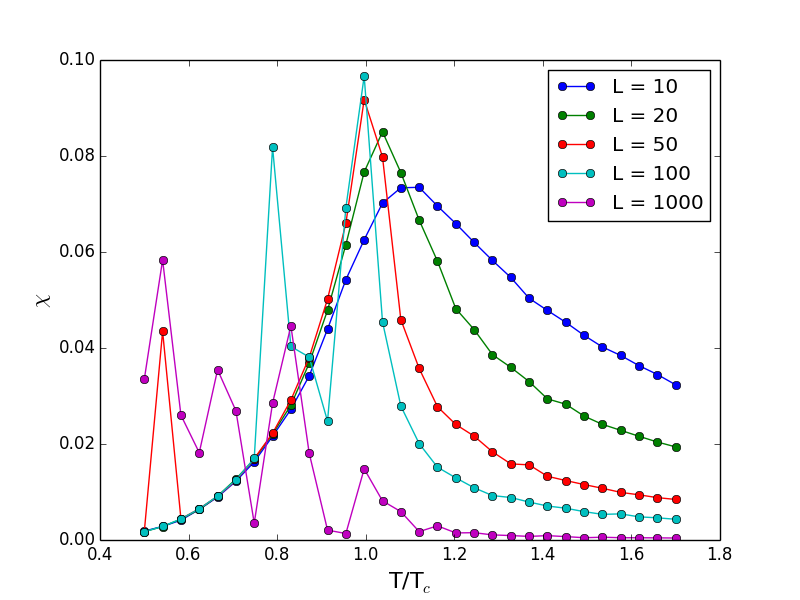
\includegraphics[width=.9\linewidth]{./images/susseptibility.png}



\section{Finite Size Scaling}
\label{sec-6}

We know that in the infinite size limit, all observables behave as \( O \propto |T - T_{c}|^{\alpha}\). To estimate the value of T$_{\text{c}}$ and the critical exponent for the magnetization (B), from our simulations, we will do a non linear fit of our data to this relation. For a system size of 50 let us run a few simulations around the critical point so that we can get a good fit it to our scaling relation.

\subsection{Job Submission}
\label{sec-6-1}

Here is a script that submits a 100 jobs at different temperatures around the critical point.
\begin{minted}[frame=lines,fontsize=\scriptsize,linenos]{python}
import matplotlib.pyplot as plt
from ising import *
import os

Ns = [50]  # System Size
T_Tcs = np.linspace(0.9, 1.1, 100)  # T/Tc
Tc = 2.268  # Onsager's Tc

for n in Ns:
    for i, T_Tc in enumerate(T_Tcs):
        T = T_Tc*Tc
        wd = 'finite-size-scaling/size-{0}/temp-{1}'.format(n, i)
        if not os.path.exists(wd): 
            os.makedirs(wd)
        write_job_script(wd=wd, n=n, s= n * 1000000, T=T, i=i)
        run_job(wd)
\end{minted}

\subsection{Fitting}
\label{sec-6-2}

Now we are ready to perform the fitting. We select 40 values on the left of the expected Onsager value for T$_{\text{c}}$ and do a nonlinear fit.

\begin{minted}[frame=lines,fontsize=\scriptsize,linenos]{python}
from __future__ import division
import numpy as np
np.set_printoptions(precision=3)
import matplotlib.pyplot as plt
from pycse import nlinfit
from ising import *

n = 50  # System Size
T_Tcs = np.linspace(0.9, 1.1, 100)  # T/Tc
Tc = 2.268  # Onsager's Tc
outfile = 'finite-size-scaling/size-{0}/temp-{1}/temp-{1}.out'

avgspins = []

for i, T_Tc in enumerate(T_Tcs):
    T = T_Tc*Tc
    indices, spins = np.loadtxt(outfile.format(n,i), unpack =True)
    spins = spins[int(len(spins)/2):]
    avgspin = np.sum(np.abs(spins)) / n ** 2 / len(spins)
    avgspins.append(avgspin)
    
# data
Ts = T_Tcs * Tc

# Let us fit the first 45 values on the left of Onsager's Tc
Ts2fit = Ts[0:40]
avgspins2fit = avgspins[0:40]

# Function to fit to
def M_fit(Ts, Tcinf, beta, a):

    M = a * np.abs((-Ts + Tcinf) / Tcinf) ** beta
    return M

# Initial guess
guess = [2.4, 0.1, 1]

pars, pint, SE = nlinfit(M_fit, Ts2fit, avgspins2fit, guess, alpha=0.05)
Tcinf, beta, a = pint

print 'T_{{c}} = {0:1.3f} (95% confidence interval = {1:1.3f} {2:1.3f}])\n'.format(pars[0], pint[0][0], pint[0][1])
print '\beta = {0:1.3f} (95% confidence interval = [{1:1.3f} {2:1.3f}])'.format(pars[1], pint[1][0], pint[1][1])

# Plotting
Tfit = np.linspace(Ts2fit.min(), Tc)
plt.plot(Ts, avgspins, 'o')
plt.plot(Tfit, M_fit(Tfit, *pars))
plt.xlabel('T$', fontsize=16)
plt.ylabel('<M$_{50}$>', fontsize=16)
plt.savefig('images/finite-size-scaling.png')
plt.show()
\end{minted}

T$_{\text{c}}$ = 2.275 (95\% confidence interval = 2.259 2.291])

$\beta$ = 0.111 (95\% confidence interval = [0.096 0.127])

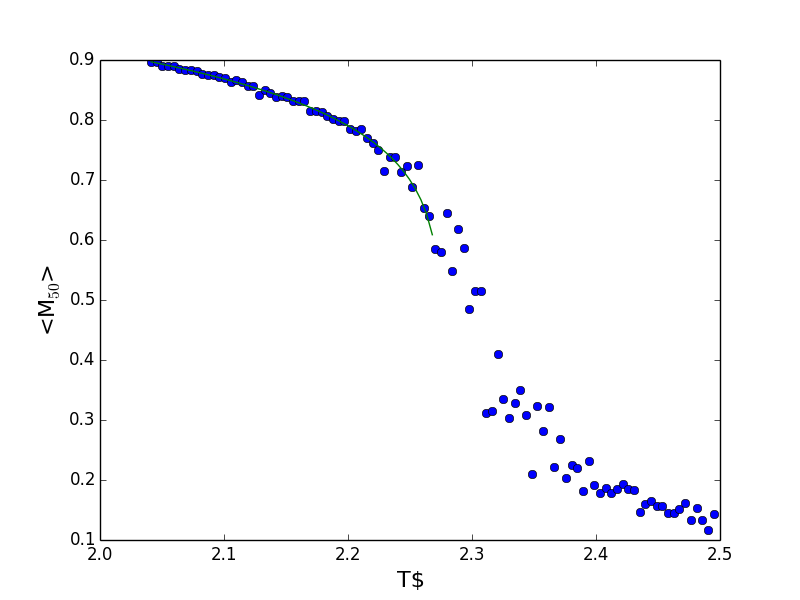
\includegraphics[width=.9\linewidth]{./images/finite-size-scaling.png}

Looks like its a pretty good fit. We almost exactly reproduce the literature values!


\section{Correlation Function}
\label{sec-7}

The correlation function is given by \(<\sigma_{i} \sigma_{j}> - <\sigma_{i}><\sigma_{j}>\). 

\begin{itemize}
\item Let us consider a spin in a 20 \texttimes{} 20 lattice, say, [i, j].

\item Now, at a given separation, r, we can have a spin in four directions, given by [i, j + r], [i, j - r], [i + r, 10], [i - r, 10].

\item At this point we can calculate the correlation function for various values of r and at different temperatures.
\end{itemize}

Here is the code that does this.

\begin{minted}[frame=lines,fontsize=\scriptsize,linenos]{python}
from __future__ import division
from ising import *
import matplotlib.pyplot as plt


n = 20 # Lattice size
nsteps = 1000000 

temperatures = [1.5, 2.268, 5.0]
# Different values of the separation
rs = np.arange(1,10, 1)

for T in temperatures:
    corr_funcs = []

    for r in rs:
        Sis, SiSjs = ising(n=n, nsteps=nsteps, correlation=True, corr_ij =[10,10], corr_r=r, T=T)
        Si_avg = sum(Sis) / nsteps
        SiSj_avg = sum(SiSjs) / nsteps
        corr_func = np.abs(SiSj_avg - Si_avg ** 2)
        corr_funcs.append(corr_func)
    plt.plot(rs, corr_funcs, 'o-', label='T = {0}'.format(T))

plt.xlabel('Separation between spins', fontsize =16)
plt.ylabel('Correlation Function', fontsize = 16)
plt.legend()
plt.savefig('images/correlation.png')
plt.show()
\end{minted}

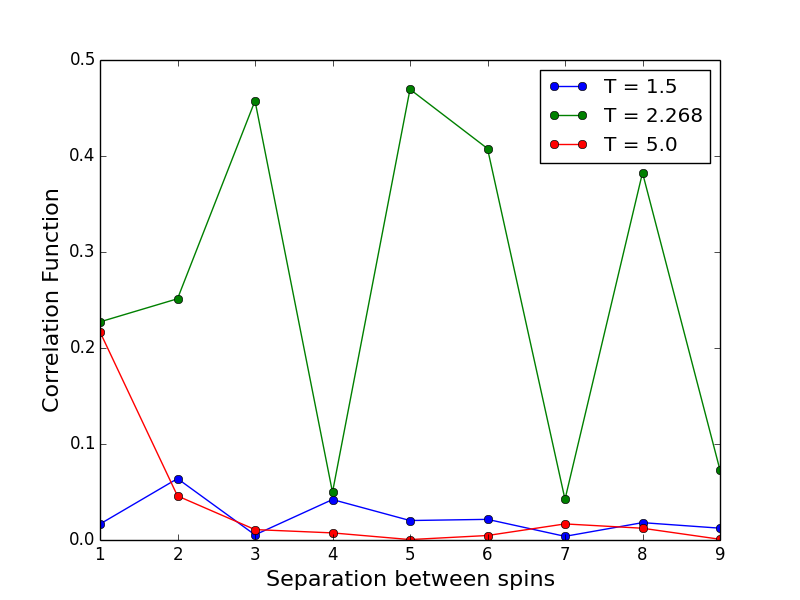
\includegraphics[width=.9\linewidth]{./images/correlation.png}

It looks like the correlation function decays pretty fast at low and high temperatures because the spin correlates the most with its nearest neighbours and there is no significant long range correlation. However, the correlation function maximum at the critical temperature and we see long range correlation, probably because of the net magnetization of the system.


\section{A little bit about Umbrella Sampling}
\label{sec-8}

Umbrella sampling is a non-Boltzmann sampling technique commonly used in systems where the ergodic behavior is hindered by the energy landscape. For example if there is an energy barrier separating two configurations of the system, it might suffer from poor sampling if Metropolis Monte Carlo is used. This is because in the Metropolis sampling, since the probability of overcoming the barrier is low, configurations on either side of the barrier may be poorly sampled, or even unsampled, by the simulaiton. For example, the melting of a solid has a barrier for phase transition, and a Metropolis simulation might not adequately sample both the solid phase and the liquid phase.

In umbrella sampling, the Boltzmann weighting for Monte Carlo sampling is replaced by a potential chosen to cancel the influence of the energy barrier present, effectively forming a reference system with the barrier removed. The energy is biased like, \( E^{\prime} = E + W \), where W is 0 for the types of configurations we are interested in, but very large for those that we are not interested in. With umbrella sampling, the Monte-Carlo simulation only visits the states we are interested in.

We didn't have time to complete the problem in Chandler 6.10, and it is not shown here.


\section{Flipping behavior of a single spin}
\label{sec-9}

We see that at high temperatures, the spin flips at short intervals. As we decrease the temperature, the spin hardly flips because the system becomes ordered.

\begin{minted}[frame=lines,fontsize=\scriptsize,linenos]{python}
from ising import *
import matplotlib.pyplot as plt
temperatures = np.linspace(1.7, 0.5, 6) * 2.26

ij = [2, 2]
for i, T in enumerate(temperatures):
    counted_spins, counted_intervals = ising(n=10,
                                             nsteps=1000000,
                                             H=0,
                                             J=1,
                                             T=T, 
                                             count_spins=True,
                                             countij=ij)
    plt.subplot(3,2,i+1)
    plt.hist(counted_intervals, 50)
    plt.locator_params(nbins=4)
    plt.title('T = {0}'.format(T))
    plt.xlabel('Flip Interval Frequency')
    plt.ylabel('No. of occurances')
plt.tight_layout()
plt.savefig('images/histograms.png')
plt.show()
\end{minted}

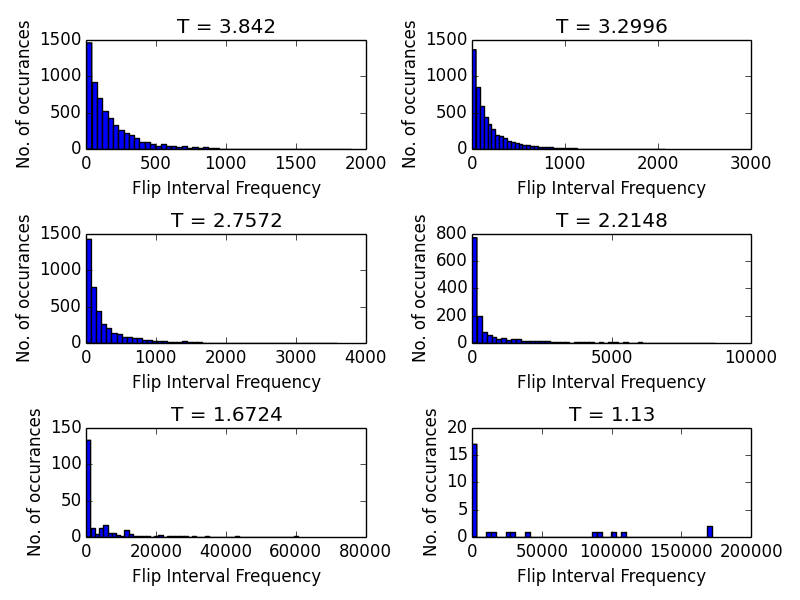
\includegraphics[width=.9\linewidth]{./images/histograms.png}
% Emacs 24.3.1 (Org mode 8.2.10)
\end{document}